\documentclass[]{article}
\usepackage{amssymb,amsmath}
\usepackage{hyperref}

\usepackage{todonotes}
\usepackage[margin=2.5cm]{geometry}
\usepackage[super]{natbib}
\bibliographystyle{unsrtnat}


\title{Information Theory and Statistical Mechanics}

\author{E. T. Jaynes\\
Washington University}
\date{July 1962}

\begin{document}

BRANDEIS UNIVERSITY SUMMER INSTITUTE\\
LECTURES IN THEORETICAL PHYSICS

K. W. Ford, \emph{\textbf{Editor}}

\begin{enumerate}
\def\labelenumi{\arabic{enumi}.}
\setcounter{enumi}{1959}
\item
  Lectures

\begin{quote}
C. Miller • P. T. Matthews • J. Schwinger • N. Fukuda • J. J. Sakurai
\end{quote}

\item Lectures
  \begin{quote}
  \emph{\textbf{Vol. 1}}
R. J. Eden • J. C. Polkinghorne • G. Källén • J. J.Sakurai
\end{quote}


\begin{quote}
\emph{\textbf{Vol. 2}}
M. E. Rose • E. C. G. Sudarshan
\end{quote}

\item
  Lectures

\begin{quote}
\emph{\textbf{Vol. 1---Elementary Particle Physics and Field Theory}} T.
Fulton • G. Kallen • J. D. Jackson • C. Fronsdal

\emph{\textbf{Vol. 2---Astrophysics and ihe Many-Uody Problem}} E. N.
Parker • J. S. Goldstein • A. A. Maiadudin • V. Anibcgaokar

\emph{\textbf{Vol. 3---Statistical Physics}} G. E. Uhlenbeck • N.
Rosenzwcig • A. J. F Siegert • E. T. Jaynes • S. Fujita
\end{quote}

\end{enumerate}

Brandeis Summer Institute 1962

STATISTICAL

PHYSICS

3

G. E. Uhlenbeck N. Hosenzweig A. J, F. Siegert E. T. Jaynes S. Fujita

\emph{\textbf{W. A.}} BENJAMIN, INC\emph{\textbf{.}} STATISTICAL PHYSICS

\begin{quote}
1962 Brandeis Lectures in Theoretical Physics, Volume 3

G. E. Uhlenbeck, N. Rosenzweig, A. J. F. Siegert, E. T. Jaynes, and C.
Fujita.
\end{quote}

In his course on SELECTED TOPICS IN STATISTICAL MECHANICS, Professor G.
E. Uhlenbeck begins with an exposition of some diagrammatic methods used
to calculate virial coefficients and the equation of state. He then
gives a detailed analysis of the mathematics of phase transition with a
soluble one-dimensional model.

The second set of lectures, by Dr. N. Rosenzweig, STATISTICAL MECHANICS
OF EQUALLY LIKELY QUANTUM SYSTEMS, is a discussion of the statistical
properties of energy levels and eigenfunctions for heavy nuclei and
complex atoms, stressing the role of time reversal and other symmetries.

Professor A. J. F. Siegert lectures on FUNCTIONAL INTEGRALS IN
STATISTICAL MECHANICS, demonstrating the utility of new techniques by
analysis of the partition function of the Ising model with long range
interactions.

Information theory has provided the long hoped for algorithm analogous
to the partition sum of equilibrium theory, for calculation of
irreversible processes. The lectures of Professor E. T. Jaynes,
INFORMATION THEORY AND STATISTICAL MECHANICS, provide an introduction to
this subject.

In the final set of lectures, Professor C. Fujita reviews and compares
the independent achievements of Van Hove and Prigogine and their
schools, in their progress toward better understanding the APPROACH TO
EQUILIBRIUM OF A MANY-PARTICLE SYSTEM.



\section*{Foreword}

It is now an established tradition of the Brandeis Summer Institute in
Theoretical Physics to have lecturers who present a systematic account
of recent research in various fields of theoretical physics. The lecture
notes have also become a part of tins tradition, and, although these are
sometimes but a first approximation to the spoken lecture, they may
serve to bring these much needed expositions to the wider audience of
physicists who may aspire to contribute to these fields.

I should like to take this opportunity to thank all those whose
participation in the Institute during the summer of 1962 helped maintain
these traditions. Particular words of appreciation are due the National
Science Foundation, for its indispensable financial support, and
Professor Kenneth Ford, who graciously carried the responsibility for
getting the notes ready for publication.

In this volume, the notes of Professor Jaynes and Professor Fujita have
been prepared by the lecturers; Professor Uhlenbeck, Dr. Rosenzweig, and
Professor Siegert have kindly checked over the notes based on their
lectures.

\begin{quote}
\emph{\textbf{\textsc{David L. Falkoff}}} Co-Director of the
\emph{\textbf{1962}} Institute
\end{quote}

\maketitle 

Notes by the lecturer

\tableofcontents

\section{Introduction}\label{introduction}

At the beginning of every problem in probability theory, there arises a
need to assign some initial probability distribution; or what is the
same thing, to ``set up an ensemble.'' This is a problem which cannot be
evaded, and for which the laws of physics give us no help. For example,
the laws of physics tell us that a density matrix
\(\rho\left( t \right)\) must vary with time according to
\(\dot{\rho} = \lbrack H,\rho\rbrack\), but they do not
tell us what function \(\rho(0)\) should be put in at the start.
Assignment of \(\rho(0)\) is, of course, a matter of free choice on our
part---it is for us to say which problem we want to solve.

The assignment of initial probabilities must, in order to be useful,
agree with the initial information we have (i.e., the results of
measurements of certain parameters). For example, we might know that at
time \(t = 0\), a nuclear spin system having total (measured) magnetic
moment \(M(0)\), is placed in a magnetic field \(H\), and the problem is
to predict the subsequent variation \(M(t)\), which presumably tends to
an equilibrium value \(M\left( \infty \right) = x_{0}H\) after a long
time. What initial density matrix for the spin system \(\rho(0)\),
should we use? Evidently, we shall want it to satisfy, at the very
least,

\begin{equation}
\text{Tr}\left( \rho(0)M_{o_{p}} \right) = M(0) \label{eqn-one}
\end{equation}

where \(M_{o_p}\) is the operator corresponding to total magnetic moment. But Eq. (\ref{eqn-one}) is very far from uniquely
specifying \(\rho(0)\). Out of the infinite number of density matrices
satisfying (\ref{eqn-one}), which should we choose as the starting point of our
calculation to predict \(M(t)\)?

Conventional quantum theory has provided an answer to the problem of
setting up initial state descriptions only in the limiting case where
measurements of a ``complete set of commuting observables'' have been
made, the density matrix \(\rho(0)\) then reducing to the projection
operator onto a pure state \(\psi(0)\) which is the appropriate
simultaneous eigenstate of all the measured quantities. But there is
almost no experimental situation in which we really have all this
information, and before we have a theory able to treat actual
experimental situations, existing quantum theory must be supplemented
with some principle that tells us how to translate, or encode, the
results of measurements into a definite state description \(\rho(0)\).
Note that the problem is not to find the \(\rho(0)\) which correctly
describes the "true physical situation." That is unknown, and always
remains so, because of incomplete information. In order to have a usable
theory we must ask the much more modest question: ``What \(\rho(0)\) best
describes our \emph{state of knowledge} about the physical situation?''

In order to emphasize that this problem really has nothing to do with
the laws of physics (and, as a corollary, that its solution will have
applications outside the field of physics), consider the following
problem. A die has been tossed a very large number \(N\) of times, and
we are told that the \emph{average} number of spots up per toss was not
3.5, as we might expect from an honest die, but 4.5. Translate this
information into a probability assignment
\(P_{n},n = 1,\ 2,\ \ldots,6\), for the \(n\)th face to come up on the
next toss.

To explain more fully what is meant by this, note that we are not asking
for an estimate of the fraction (i.e., the relative frequency) of tosses
which give \(n\) spots There is, indeed, a connection between the
probability and the frequency, which we will derive later. But the
problem stated is to reason as best we can about the \emph{individual}
case. The probability \(P_{n}\) must therefore be interpreted in the
so-called "subjective" sense; it is only a means of describing how
strongly we \emph{believe} that the \(n\)-th face will come up in the
next toss.

To state the problem more drastically, imagine that we are offered
several bets, at various odds, on various values of \(n\), and we are
compelled to accept one of these bets. The probabilities \(P_{n}\) are
the basic raw material from which we decide which one to accept. This is
typical of many practical problems faced by the scientist, the engineer,
the statistician, the politician; and indeed all of us. We are
continually faced with situations where some definite decision must be
made \emph{now}, even though we do not have all the information we might
like.
%
\begin{align}
\sum_{n = 1}^{6} P_{n} = & 1  \label{eqn-two} \\
\sum_{n = 1}^{6} nP_{n} = & 4.5 \label{eqn-three}
\end{align}
%
\begin{figure}
    \centering
    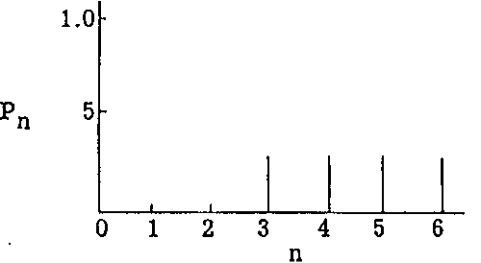
\includegraphics[width=3.20866in,height=1.75197in]{media/image1.jpeg}
    \caption{}
    \label{fig-one}
\end{figure}
%
\begin{figure}
    \centering
    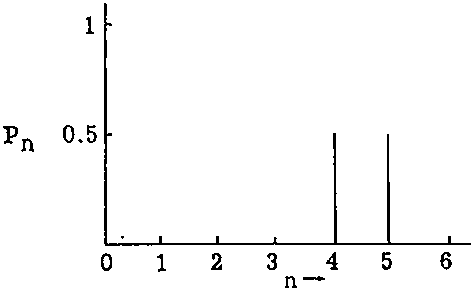
\includegraphics[width=3.16142in,height=2in]{media/image2.png}
    \caption{}
    \label{fig-two}
\end{figure}
%
where (\ref{eqn-three}) is analogous to (\ref{eqn-one}). A possible solution of (\ref{eqn-two}) and (\ref{eqn-three}) is indicated
in Fig. \ref{fig-one}; we could take \(P_{4} = P_{5} = 1/2\), all other
\(P_{n} = 0\), This agrees with all the given data. But our common sense
tells us it is not a \emph{reasonable} assignment. The assignment of
Fig. \ref{fig-two} is evidently a more honest description of what we know. But even
this is not reasonable---nothing in the data tells us that n = 1, 2 are
impossible events. In Fig. \ref{fig-two}, we are still jumping to conclusions not
warranted by the available evidence. Evidently, it is unreasonable to
assign probability zero to any situation unless our data really rules
out that case. If we assign \(P_{1} > 0\), \(P_{2} > 0\), then in order
to keep the average at 4.5, we shall have to give some increased weight
to the cases \(n = 5,\ 6\). Figure \ref{fig-three} shows an assignment that agrees
with the data and does not ignore any possibility. But it still seems
unreasonable to give the case \(n = 6\) such exceptional treatment.
Figure \ref{fig-four} represents what we should probably call a
\begin{figure}
    \centering
    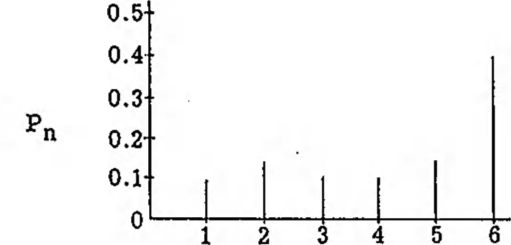
\includegraphics[width=3.39764in,height=1.64567in]{media/image3.jpeg}
    \caption{}
    \label{fig-three}
\end{figure}
\begin{figure}
    \centering
    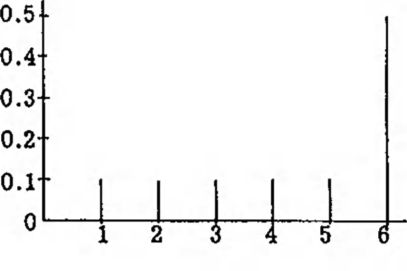
\includegraphics[width=2.71319in,height=1.81042in]{media/image4.jpeg}
    \caption{}
    \label{fig-four}
\end{figure}
backward
step---nothing in the data of the problem indicates any reason for such
an uneven treatment. A reasonable assignment \(P_{n}\) must not only
agree with the data and must not ignore any possibility---but
it must also not give undue emphasis to any possibility. The \(P_{n}\)
should vary as smoothly as possible, in some sense. One criterion of
"smoothness" might be that adjacent differences \(P_{n + 1} - P_{n}\)
should be constant; and, indeed, there is a solution with that property.
It is given by \(P_{n} = (12n - 7)/210\) and
\begin{figure}
    \centering
    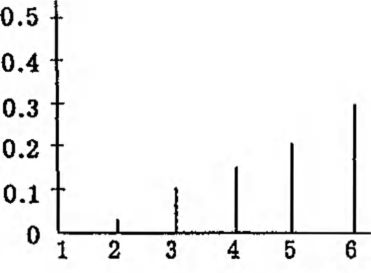
\includegraphics[width=2.48031in,height=1.82283in]{media/image5.jpeg}
    \caption{}
    \label{fig-five}
\end{figure}
is
shown in Fig. \ref{fig-five}. This is evidently the most reasonable probability
assignment so far. But there is a limit to how high an average you can
get with this linear variation of \(P_{n}\). If we took the extreme
case, \(P_{n} = (const.)(n - 1)\), we should again violate one of our
principles because \(P_{1} = 0\), and the average would be only
\(\sum_{n}^{}{P_{n} = 70/15} = 4.67\). Suppose the data of the problem
had been changed so that the average is to be 4.7 instead of 4.5. Then
there is no straight-line solution satisfying \(P_{n} \geq 0\). The
\(P_{n}\) must lie on some concave curve, as in Fig. 6. But the
principles by which we reason
surely
\begin{figure}
    \centering
    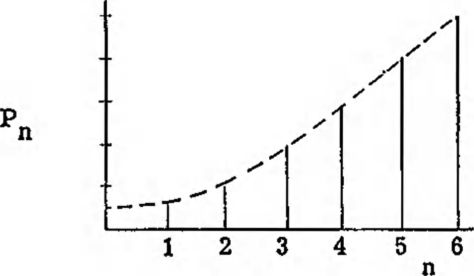
\includegraphics[width=3.16535in,height=1.84252in]{media/image6.jpeg}
    \caption{}
    \label{fig-six}
\end{figure}
%
are the same whether the data specify 4.5 or 4.7; so it appears that a
result qualitatively such as Fig. \ref{fig-six} should be used also when
\(n = 4.5\).

This is about as far as qualitative reasoning can take us, and I have carried the argument through on that basis in order to show how ordinary common sense leads us to a result that has all the important features of the quantitative solution given below. The probability assignment $P _{ n }$ which most honestly describes what we know is the one that is as smooth and "spread out" as possible subject to the data. It is the most conservative assignment in the sense that it does not permit one to draw any conclusions not warranted by the data.

This suggests that the problem is a variational one; we need a measure of the "spread" of a probability distribution which we can maximize, subject to constraints which represent the available information. It is by now amply demonstrated by many workers that the "information measure" introduced by Shannon\citep{Shannon-mathematical48} has special properties of consistency and uniqueness which make it \emph{the} correct measure of "amount of uncertainty" in a probability distribution. This is, of course, the expression
%
\begin{equation}
S_{I} = - \sum_{i}^{} p_{i}\log p_{i}
\end{equation}
%
which, \emph{for some distributions} and \emph{in some physical situations}, has long been recognized as representing entropy. However, we have to emphasize that "information-theory entropy" $S _{ I }$ and the experimental thermodynamic entropy $S _{e}$ are entirely different concepts. Our job cannot be to \emph{postulate} any relation between them; it is rather to \emph{deduce} whatever relations we can from known mathematical and physical facts. Confusion about the relation between entropy and probability has been one of the main stumbling blocks in developing a general theory of irreversibility.

\section{The General Maximum-Entropy Formalism}\label{the-general-maximum-entropy-formalism}

To generalize the above problem somewhat, suppose that the quantity
\(x\) can take on the values \((x_1, x_2, \dots x_n)\) where $n$ can be finite or
infinite, and that the average values of several functions $(f_1(x), f_2(x), \dots f_m(x)$ are given, where $m < n$. The problem is to find the probability assignment $p_i =
p(x_i)$ which satisfies the given data: $p_i \geq 0$,
%
\begin{equation}
\sum_{i = 1}^{n} p_{i} = 1 \label{eqn-five}
\end{equation}
\begin{equation}
\sum_{i = 1}^{n}  p_{i}f_{k}\left( x_{i} \right) = \left\langle f_{k}(x) \right\rangle = F_{k} \quad k = 1,2,\ldots,m \label{eqn-six}
\end{equation}
%
and, subject to (\ref{eqn-five}) and (\ref{eqn-six}), maximizes the entropy
%
\begin{equation}
S_{I} = - \sum_{i = 1}^{n} p_{i}\log p_{1} \label{eqn-seven}
\end{equation}
%
The solution to this mathematical problem can be found immediately by
the method of Lagrangian multipliers, and special cases are given in
every statistical mechanics textbook. This method has the merit that it
leads immediately to the answer, but the weakness that it does not make
it obvious whether one obtains a true absolute maximum of \(S_{I}\). The
following argument establishes this important result more rigorously.
Let \(\left( p_{1}\ldots p_{n} \right)\) and
\(\left( u_{1}\ldots u_{n} \right)\) be any two possible probability
distributions over the \(x_{1};\) i.e.,
\(p_{i} \geq 0,u_{i} \geq 0,i = 1,2,\ldots\) n and
%
\begin{equation}
\sum_{i = 1}^{n} p_{1} = \sum_{i = 1}^{n} u_{i} = 1
\end{equation}
%
Then, by using the fact that
\(logx \geq \left( 1 - x^{- 1} \right),\) with equality if and only if
\(x = 1,\) we find the following:

\paragraph{Lemma}

\begin{equation}
\sum_{i = 1}^{n}  p_{i}\log\frac{p_{i}}{u_{i}} \geq \sum_{i = 1}^{n}  p_{i}\left( 1 - \frac{u_{i}}{p_{i}} \right) = 0 \label{eqn-nine}
\end{equation}
%
with equality if and only if \(p_{i} = u_{i},i = 1,2,\ldots n\). Now
make the choice
%
\begin{equation}
u_{i} = \frac{1}{Z\left( \lambda_{1}\ldots\lambda_{m}) \right.\ }\exp\left( - \lambda_{1}f_{1}\left( x_{i} \right) - \ldots - \lambda_{m}f_{m}\left( x_{i} \right) \right) \label{eqn-ten}
\end{equation}
%
where \(\lambda_{1}\ldots\lambda_{m}\) are fixed constants, and
%
\begin{equation}
Z\left( \lambda_{1}\ldots\lambda_{m} \right) \equiv \sum_{i = 1}^{n}  \exp\left( - \lambda_{1}f_{1}\left( x_{1} \right) - \ldots - \lambda_{m}f_{m}\left( x_{i} \right) \right) \label{eqn-eleven}
\end{equation}
%
will be called the ``partition function.'' Substituting (\ref{eqn-ten}) into (\ref{eqn-nine})
results in the inequality

\begin{align*}
\sum_{i = 1}^{n}   p_{i}\log p_{i} \geq \sum_{i = 1}^{n}   p_{i}\log u_{i} = &  - \sum_{i = 1}^{n}   p_{i}\left\lbrack \lambda_{1}f_{1}\left( x_{i} \right) + \ldots \right. \\
 & \left.  + \lambda_{m}f_{m}\left( x_{i} \right) \right\rbrack - \log Z\left( \lambda_{1}\ldots\lambda_{m} \right) \\
\end{align*}
%
or
%
\begin{equation}
S_{I} \leq  \log Z\left( \lambda_{1}\ldots\lambda_{m} \right) + \sum_{k = 1}^{m} \lambda_{k}\left\langle f_{k} \right\rangle \label{eqn-twelve}
\end{equation}
%
Now let the distribution \(p_{i}\) vary over the class of all possible
distributions that satisfy (\ref{eqn-six}). The right-hand side of (\ref{eqn-twelve}) remains
fixed, and (\ref{eqn-twelve}) shows that \(S_{I}\) attains its maximum possible value
%
\begin{equation}
\left( S_{I} \right)_{\max} =  \log Z + \sum_{k = 1}^{m} \lambda_{k}\left\langle f_{k} \right\rangle \label{eqn-thirteen}
\end{equation}
%
if and only if \(p_{i}\) is taken as the generalized canonical
distribution
(\ref{eqn-ten}). It only remains to choose the unspecified constants
\(\lambda_{k}\) so that (\ref{eqn-six}) is satisfied. This is the case, as one
readily verifies, if the \(\lambda_{k}\) are determined in terms of the
given data \(F_{k} = \left\langle f_{k} \right\rangle\) by
%
\begin{equation}
\left\langle f_{k} \right\rangle = - \frac{\partial}{\partial\lambda_{k}} \log Z\left( \lambda_{1}\ldots\lambda_{m} \right)\ \quad  k = 1,2,\ldots,m \label{eqn-fourteen}
\end{equation}
%
We now survey rapidly the main formal properties of the distribution
found. The maximum attainable entropy (\ref{eqn-thirteen}) is some function of the given
data:
%
\begin{equation}
\left( S_{I} \right)_{\max} = S\left( \left\langle f_{1} \right\rangle,\ldots\left\langle f_{m} \right\rangle \right)
\end{equation}
%
and, by using (\ref{eqn-thirteen}) and (\ref{eqn-fourteen}), we find
%
\begin{equation}
\frac{\partial S}{\partial\left\langle f_{k} \right\rangle} = \lambda_{k}\ k = 1,2,\ldots,m \label{eqn-sixteen}
\end{equation}
%
Regarding, in (\ref{eqn-fourteen}), the \(\left\langle f_{k} \right\rangle\) expressed
as functions of \(\left( \lambda_{1}\ldots\lambda_{m} \right)\) we find,
on differentiating, the reciprocity law
%
\begin{equation}
\frac{\partial\left\langle f_{k} \right\rangle}{\partial\lambda_{j}} = \frac{\partial\left\langle f_{j} \right\rangle}{\partial\lambda_{k}} = - \frac{\partial^{2}}{\partial\lambda_{k}\partial\lambda_{j}} \log Z = A_{jk} \label{eqn-seventeen}
\end{equation}
%
while by the same argument, if we regard \(\lambda_{k}\) in (\ref{eqn-sixteen})
expressed as a function of \(\left\langle f_{1} \right\rangle\ldots\left\langle f_{m} \right\rangle,\) we find a corresponding law
%
\begin{equation}
\frac{\partial\lambda_{k}}{\partial\left\langle f_{j} \right\rangle} = \frac{\partial\lambda_{j}}{\partial\left\langle f_{k} \right\rangle} = \frac{\partial^{2}S}{\partial\left\langle f_{j} \right\rangle\partial\left\langle f_{k} \right\rangle} = B_{jk} \label{eqn-eighteen}
\end{equation}
%
Comparing (\ref{eqn-seventeen}) and (\ref{eqn-eighteen}) and remembering the chain rule for
differentiating,
%
\begin{equation*}
\frac{\partial\left\langle f_{j} \right\rangle}{\partial\left\langle f_{k} \right\rangle} = \sum_{ \ell}^{} \frac{\partial\left\langle f_{j} \right\rangle}{\partial\lambda_{ \ell}}\frac{\partial\lambda_{ \ell}}{\partial\left\langle f_{k} \right\rangle} = \delta_{jk}
\end{equation*}
%
we see that the second derivatives of \(S\) and of $\log Z$ yield
inverse matrices:
%
\begin{equation}
A = B^{- 1}
\end{equation}
%
The functions \( \log Z\left( \lambda_{1}\ldots\lambda_{n} \right)\) and
\(S\left( \left\langle f_{1} \right\rangle\ldots\left\langle f_{n} \right\rangle \right)\)
are equivalent in the sense that each gives full information about the
probability distribution; indeed (\ref{eqn-thirteen}) is just the Legendre
transformation that takes us from one representative function to the
other.

The reciprocity law (\ref{eqn-seventeen}) acquires a deeper meaning when we consider the
``fluctuations'' in our probability distribution. Using the distribution
(\ref{eqn-ten}), a short calculation shows that the second central moments of the
distribution of the \(f_{k}(x)\) are given by
%
\begin{align}
\left\langle \left( f_{k} - \left\langle f_{k} \right\rangle \right)\left( f_{ \ell} - \left\langle f_{ \ell} \right\rangle \right) \right\rangle & = \left\langle f_{k}f_{ \ell} \right\rangle & \  - \left\langle f_{k} \right\rangle\left\langle f_{ \ell} \right\rangle \nonumber \\
& \label{eqn-twenty} \\
 & = & \frac{\partial^{2}}{\partial\lambda_{k}\partial\lambda_{ \ell}} \log Z \nonumber
\end{align}
%
and so, comparing with (\ref{eqn-seventeen}) , there is a universal relation between the
``fluctuations'' of the \(f_{k}\) and the ``compliance coefficients''
\(\partial\left\langle f_{k} \right\rangle/\partial\lambda_{ \ell}:\)
%
\begin{equation}
\left\langle f_{k}f_{l} \right\rangle - \left\langle f_{k} \right\rangle\left\langle f_{ \ell} \right\rangle = - \frac{\partial\left\langle f_{k} \right\rangle}{\partial\lambda_{ \ell}} = - \frac{\partial\left\langle f_{ \ell} \right\rangle}{\partial\lambda_{k}} \label{eqn-twenty-one}
\end{equation}
%
Likewise, higher derivatives of
\( \log Z\left( \lambda_{1}\ldots\lambda_{n} \right)\) yield higher central
moments of the \(f_{k}\), in a manner analogous to (\ref{eqn-twenty}), and a hierarchy
of fluctuation laws similar to (\ref{eqn-twenty-one}).
%
In addition to their dependence on \(x\), the functions \(f_{k}\) may
depend on another parameter, \(\alpha.\) The partition function will
then also have an explicit dependence on \(\alpha\) :
%
\begin{equation}
Z\left( \lambda_{1}\ldots\lambda_{m};\alpha \right) \equiv \sum_{i = 1}^{n}  \exp\left( - \lambda_{1}f_{1}\left( x_{i};\alpha \right) - \ldots - \lambda_{m}f_{m}\left( x_{i};\alpha \right) \right)
\end{equation}
%
and a short calculation shows that the expected derivatives
%
\begin{equation*}
\left\langle \frac{\partial f_{k}}{\partial\alpha} \right\rangle
\end{equation*}
%
satisfy the relations
%
\begin{equation}
\sum_{k = 1}^{m} \lambda_{k}\left\langle \frac{\partial f_{k}}{\partial\alpha} \right\rangle = - \frac{\partial}{\partial\alpha} \log Z = - \frac{\partial S}{\partial\alpha} \label{eqn-twenty-three}
\end{equation}
%
If several parameters \(\alpha_{1}\ldots\alpha_{r}\) are present, a
relation of this form will hold for each of them.

Finally, we note an important variational property which generalizes
(\ref{eqn-sixteen}) to the case where we have also variations in the parameters
\(\alpha_{1}\ldots\alpha_{r}.\) Let
\(Z = Z\left( \lambda_{1}\ldots\lambda_{m};\alpha_{1}\ldots\alpha_{r} \right),\)
and consider an arbitrary small change in the problem, where the given
data \(\left\langle f_{k} \right\rangle\) and the parameters
\(\alpha_{j}\) are changed by small amounts
\(\delta\left\langle f_{k} \right\rangle/\delta\alpha_{j}\) This will
lead to a change \(\delta\lambda_{k}\) in \(\lambda_{k}\). From (\ref{eqn-thirteen}),
the maximum attainable entropy is changed by

\begin{align}
\delta S = & \sum_{k = 1}^{m}  \frac{\partial  \log Z}{\partial\lambda_{k}}\delta\lambda_{k} + \sum_{j = 1}^{r}  \frac{\partial  \log Z}{\partial\alpha_{j}}\delta\alpha_{j} \nonumber \\
\label{eqn-twenty-four} \\
 & \  + \sum_{k = 1}^{m}  \left\langle f_{k} \right\rangle\delta\lambda_{k} + \sum_{k = 1}^{m}  \lambda_{k}\delta\left\langle f_{k} \right\rangle \nonumber
\end{align}

The first and third terms cancel by virtue of (\ref{eqn-fourteen}). Then, using (\ref{eqn-twenty-three}), we
have
%
\begin{equation}
\delta S = - \sum_{j = 1}^{r} \sum_{k = 1}^{m} \lambda_{k}\left\langle \frac{\partial f_{k}}{\partial\alpha_{j}} \right\rangle\delta\alpha_{j} + \sum_{k = 1}^{m} \lambda_{k}\delta\left\langle f_{k} \right\rangle
\end{equation}
%
Now we can write
%
\begin{equation}
\sum_{j = 1}^{r} \left\langle \frac{\partial f_{k}}{\partial\alpha_{j}} \right\rangle\delta\alpha_{j} = \left\langle \sum_{j = 1}^{r}  \frac{\partial f_{k}}{\partial\alpha_{j}}\delta\alpha_{j} \right\rangle = \left\langle \delta f_{k} \right\rangle
\end{equation}
%
and so finally
%
\begin{equation}
\delta S = \sum_{k = 1}^{m} \lambda_{k}\left\lbrack \delta\left( f_{k} \right\rangle - \left\langle \delta f_{k} \right\rangle \right\rbrack
\end{equation}
%
or
%
\begin{equation}
\delta S = \sum_{k = 1}^{m} \lambda_{k}\delta Q_{k} \label{eqn-twenty-eight}
\end{equation}
%
where
%
\begin{equation}
\delta Q_{k} \equiv \delta\left\langle f_{k} \right\rangle - \left\langle \delta f_{k} \right\rangle \label{eqn-twenty-nine}
\end{equation}

In general \(\delta Q_{k}\) is not an exact differential; i.e., there is
no function
\(Q_{k}\left( \lambda_{1}\ldots\lambda_{m};\alpha_{1}\ldots\alpha_{r} \right)\)
which yields \(\delta Q_{k}\) by differentiation. But (28) shows that
\(\lambda_{k}\) is an integrating factor such that
\(\sum_{k} \lambda_{k}\delta Q_{k}\) is the exact
differential of some ``state function''
\(S\left( \lambda_{1}\cdots\lambda_{m};\alpha_{2}\cdots\alpha_{r} \right)\).

All the above relations, (\ref{eqn-ten}) to (\ref{eqn-twenty-nine}), are elementary consequences of
maximizing the information theory entropy subject to constraints on
average values of certain quantities. Although they bear a strong formal
resemblance to the rules of calculation provided by statistical
mechanics, they make no reference to physics, and, therefore, they must
apply equally well to any problem, in or out of physics, where the
situation can be described by (\ref{eqn-one}) enumerating a discrete set of
possibilities and by (\ref{eqn-two}) specifying average values of various
quantities. The above formalism has been applied also to problems in
engineering\citep{Jaynes-decipherability59} and economics.\citep{Jaynes-engineering63}

In most problems, interest centers on making the best possible
predictions for a \emph{specific} situation, and we are not really
interested in properties of any ensemble, real or imaginary. (For
example, we want to predict the magnetization \(M(t)\) of the
\emph{particular} spin system that exists in the laboratory.) In this
case, as already emphasized, the maximum-entropy probability assignment
\(p_{i}\) cannot be regarded as describing any objectively existing
state of affairs; it is only a means of describing a state of knowledge
in a way that. is ``maximally noncommital'' by a certain criterion.

The above equations then represent simply the best predictions we are
able to make on the given information. We are not entitled to assert
that the predictions must be ``right,'' only that to make any better
ones, we should need more information than was given. However, in cases
where it makes sense to imagine \(x_{i}\) as being the result of some
random experiment which can be repeated many times, a somewhat more
``objective'' interpretation of this formalism is possible, which in
its essentials was given already by Boltzmann. We are given the same
average values \(\left\langle f_{k}(x) \right\rangle\) as before, but we
are now asked a different question. If the random experiment is repeated
\(N\) times, the result \(x_{i}\) will be obtained \(m_{i}\) times,
\(1 = 1,2,\ldots,n,\) We are to make the best estimates of the numbers
\(m_{i}\) on the basis of this much information. The knowledge of
average values tells us that
%
\begin{equation}
\sum_{i = 1}^{n} \frac{m_{i}}{N}f_{k}\left( x_{i} \right) = \left\langle f_{k} \right\rangle\ k = 1,2,\ldots,m \label{eqn-thirty}
\end{equation}
%
and, of course,
%
\begin{equation}
\sum_{i = 1}^{n} \frac{m_{i}}{N} = 1 \label{eqn-thirty-one}
\end{equation}
%
Equations (\ref{eqn-thirty}) and (\ref{eqn-thirty-one}) do not uniquely determine the \(m_{i}\) if
\(m < n - 1,\) and so again it is necessary to introduce some additional
principle, which now amounts to stating what we mean by the ``best''
estimate. The following criterion seems reasonable. In \(N\) repetitions
of the random experiment, there are \emph{a priori} \(n^{N}\)
conceivable results, since each trial could give independently any of
the results \(\left( x_{1},x_{2},\ldots,x_{n} \right)\). But for given
\(m_{i}\), there are only \(W\) of these possible, where
%
\begin{equation}
W \equiv \frac{N!}{m_{1}!\ldots m_{n}!} = \frac{N!}{\left( Ng_{1} \right)!\left( Ng_{2} \right)!\ldots\left( Ng_{n} \right)!} \label{eqn-thirty-two}
\end{equation}
%
and
%
\begin{equation}
g_{i} = \frac{m_{i}}{N}\ i = 1,2,\ldots,n
\end{equation}
%
is the \emph{relative frequency} with which the result \(x_{i}\) is obtained.
Which cholce of the \(g_{i}\) can happen in the greatest number of ways?
If we have to guess the frequencies on the basis of no more information
than (\ref{eqn-thirty}) it seems that a reasonable criterion is to ask what
choice will maximize (\ref{eqn-thirty-two}) while agreeing with (\ref{eqn-thirty}). Now in the limit of
large \(N\), we have by the Stirling formula,
%
\begin{align}
\lim_{N \rightarrow \infty} \frac{1}{N}\log W & \  = \lim_{N \rightarrow \infty} \frac{1}{N}\log\left\lbrack
\frac{N!}{\left( Ng_{1} \right)!\ldots\left( Ng_{n} \right)!} \right\rbrack \nonumber \\
\label{eqn-thirty-four}\\
 & \  = - \sum_{i = 1}^{n}   g_{i}\log g_{i} \nonumber
\end{align}
%
and so, if we are to estimate limiting frequencies in an indefinitely
large number of trials, we have in (\ref{eqn-thirty}) and (\ref{eqn-thirty-four}) formulated exactly the
same mathematical problem as in (\ref{eqn-six}) and (\ref{eqn-seven}). The same solution (\ref{eqn-ten}) and
formal properties, Eqs, (\ref{eqn-eleven}) to (\ref{eqn-twenty-nine}), follow immediately, and we have an
alternative interpretation of the maximum-entropy formalism: the
probability \(p_{i}\) which information theory assigns to the event
\(x_{i}\) at a \emph{single} trial is numerically equal to an estimate
of the relative frequency \(g_{i}\) of this result in an indefinitely
large number of trials, obtained by enumerating all cases consistent
with our knowledge, and placing our bets on the situation that can
happen in the greatest number of ways. Thus, for example, the
fluctuation laws (\ref{eqn-twenty-one}) describe, on the one hand, our uncertainty as to
the unknown true values of \(f_{k}(x)\) in a specific instance; on the
other hand, they give the best estimates we can make of the
\emph{average} departures from \(\left\langle f_{k} \right\rangle\) in
many repetitions of the experiment, by the criterion of placing our bets
on the situation that can happen in the greatest number of ways. Two
points about these interpretations should be noted:

\begin{enumerate}

\item
  In most practical problems, repeated repetition of the experiment is
  either impossible or not relevant to the real problem, which is to do
  the best we can with the \emph{individual} case. Thus if one were to
  insist, as has sometimes been done, that only the second
  interpretation is valid, the result would be to deny ourselves the use
  of this formalism in most of the problems where it is helpful.
\item
  The argument leading from the averages (\ref{eqn-thirty}) to the estimate of
  frequencies \(g_{i}\) was not deductive reasoning, but only plausible
  reasoning. Consequently, we are not entitled to assert that the
  estimates \(g_{i}\) \emph{must} be right; only that, in order to make
  any better estimates, we should need more information. Thus the
  apparently greater ``objectivity'' of the second interpretation is to
  a large extent illusory.
\end{enumerate}

\section{Application to Equilibrium Thermodynamics}

We apply the formalism of the preceding section to the following situation: $m =1$, $f_{1}\left( x _{ j }, \alpha\right)= E _{ i }( V ) .$ The parameter $V$ (volume)
and the expectation value of the energy of the system $\langle E\rangle$ are given. The partition function is
\begin{equation}
Z(\lambda, V) \equiv \sum_{i=1}^{\infty} e^{-\lambda E_{i}(V)}
\end{equation}
Then, by (\ref{eqn-fourteen}), $\lambda$ is determined from
\begin{equation}
\langle E\rangle=-\frac{\partial}{\partial \lambda} \log Z
\end{equation}
and, as a special case of (\ref{eqn-twenty-three}) we have
\begin{equation}
\lambda\left\langle\frac{\partial E}{\partial V}\right\rangle=-\frac{\partial}{\partial V} \log Z
\end{equation}
But $-\langle\partial E / \partial V\rangle=\langle P\rangle$ is the maximum-entropy estimate of pressure, and so the predicted equation of state is
\begin{equation}
\langle P \rangle=\frac{1}{\lambda} \frac{\partial}{\partial V} \log Z
\end{equation}
To identify the temperature and entropy, we use the general variational property (\ref{eqn-twenty-eight}). A small change $\delta V$ in volume will change the energy levels by $\delta E _{ i }=\left(\partial E _{ i } / \partial V \right) \delta V$, and if this is carried out infinitely slowly (i.e., reversibly), the ``adiabatic theorem'' of quantum mechanics tells us that the probabilities $p _{ i }$ will not be changed. So, the maximum-entropy estimate of the work done is
\begin{equation}
\delta W=-\langle\delta E\rangle
\end{equation}
Of course, the given $\langle E\rangle$ is interpreted as the thermodynamic energy function $U$. In addition to the change $\delta V$, we allow a small reversible heat flow $\delta Q$, and by the first law, the net change in energy is $\delta U =\delta Q -\delta W$, or 
%
\begin{equation}
\text{Equation Missing from Original} \label{eqn-forty}    
\end{equation}
%
Thus, if $f_{k}$ is the energy, then the $\delta Q_{k}$ defined by (\ref{eqn-twenty-nine}) is the predicted heat flow in the ordinary sense. Equation (\ref{eqn-twenty-eight}) shows that for \emph{any} quantity $f_{k}$, there is a quantity $\delta Q_{k}$ formally analogous to heat. 

In the present case (\ref{eqn-twenty-eight}) reduces to
\begin{equation}
\delta S(\langle E\rangle, V)=\lambda \delta Q \label{eqn-forty-one}
\end{equation}
Now the Kelvin temperature is defined by the condition that $(1 / T)$ is the integrating factor for infinitesimal reversible heat in closed systems and the experimental entropy $S_{e}$ is defined as the resulting state function. So from (\ref{eqn-forty-one}) the predicted temperature $T^\prime$ and experimental entropy $S _{ e }^{\prime}$ are given by
%
\begin{align}
\lambda= & \frac{1}{ kT ^{\prime}} \\
S _{ e }^{\prime}= & kS (\langle E \rangle, V )= k \left( S _{ I }\right)_{\max }
\end{align}

The presence of Boltzmann's constant k merely indicates the particular practical units in which we choose to measure temperature and entropy. For theoretical discussions, we may as well adopt units such that $k=1$.

All that we have shown so far is that the general maximum entropy formalism leads automatically to definitions of quantities \emph{analogous} to those of thermodynamics. This is, of course, as far as any mathematical theory can go; no amount of mathematics can prove anything about experimental facts. To put it differently, before we can establish any connection between our theoretical entropy $S_{e}^{\prime}$ and the experimentally measured quantity $S_{e}$, we have to introduce some physical assumption about what the result of an experiment would in fact be:

\paragraph{Physical assumption} The equilibrium thermodynamic properties of a system, as measured experimentally, agree with the results calculated by the usual methods of statistical mechanics; i.e., from the canonical or grand canonical ensemble appropriate to the problem. \begin{equation} \label{eqn-forty-four}\end{equation}


This assumption has proved correct in every case where one has succeeded in carrying out the calculations, and its universal validity is taken so much for granted nowadays that authors of textbooks no longer list it as an assumption. But strictly speaking, all we can prove here is that systems conforming to this assumption will also conform to various other statements made below.

If we accept (\ref{eqn-forty-four}), then the identification of entropy is complete, and connection between information theory entropy and experimental entropy for the present problem can be stated as a theorem.

\paragraph{Theorem}: Let $p _{i} \equiv  \text{prob} \left( E _{ i }\right)$ be any probability assignment which conforms to the data in the sense that $\langle E \rangle=\sum_{ i } p _{ i } E _{ i }$ is the
measured energy. Let $S_{I} \equiv-\sum p_{i} \log p_{i}$ be the corresponding information theory entropy, and $S _{e}$ be the experimentally measured entropy for the system. The additive constant is chosen so that at zero temperature $S_{e}=\log n$, where $n$ is the degeneracy of the ground state, and let $S_{e}$ be expressed in units such that Boltzmann's constant $k \equiv 1$. Then
\begin{equation}
S _{ I } \leq S _{ e }
\end{equation}
with equality if and only if $p _{ i }$ is chosen as the canonical distribution
\begin{equation}
p_{i}=\frac{1}{Z} \exp \left(-\lambda E_{i}(V)\right) \label{eqn-forty-six}
\end{equation}
This is the physical meaning, for the present problem, of the general inequality (\ref{eqn-twelve}). Obviously, the above statement can be greatly generalized; we can introduce more degrees of freedom in addition to $V$, we can consider open systems, where the number of molecules can change, and we can use the grand canonical ensemble, etc. The corresponding statement will still hold; over all probability assignments that agree with the data in the aforementioned sense, the information theory entropy attains an absolute maximum, equal to the experimental entropy, if and only if $p _{ i }$ is taken as the appropriate canonical or grand canonical distribution. 

\paragraph{Remarks:} 

\begin{enumerate}
    
\item  We have taken $\langle E \rangle$ as the given quantity. In practice, it is usually the temperature that is measured. To treat the temperature as the observable, one must regard the system of interest to be in contact with a heat reservoir, with which it may exchange energy and which acts as a thermometer. Detailed analysis of the resulting system (given in reference\citep{Jaynes-information57}) leads to the same probability assignments as we have found with
$\langle E \rangle$ as the
given datum.

\item  If not only $\langle E\rangle$ is known, but also the accuracy of the measurement, as given for example by $\left\langle E^{2}\right\rangle$, then this information may be incorporated into the problem by taking $f_{1}\left(x_{1}, \alpha\right)=$ $E _{1}( V ), f _{2}\left( x _{ 1 }, \alpha\right)= E _{ i }^{2}( V ) .$ The partition function (\ref{eqn-eleven}) becomes 
\begin{equation}
Z \left(\lambda_{1}, \lambda_{2}, V \right)=\sum_{ i } \exp \left[-\lambda_{1} E _{ i }( V )-\lambda_{2} E _{ i }^{2}( V )\right]
\end{equation}
and from (\ref{eqn-fourteen}),
\begin{equation}
\langle E \rangle=-\frac{\partial}{\partial \lambda_{1}} \log Z \quad\left\langle E ^{2}\right\rangle=-\frac{\partial}{\partial \lambda_{2}} \log Z
\end{equation}
The fluctuation theorem (\ref{eqn-twenty-one}) then gives the relation
\begin{equation}
\left\langle E^{3}\right\rangle-\langle E\rangle\left\langle E^{2}\right\rangle=-\frac{\partial(E\rangle}{\partial \lambda_{2}}=-\frac{\partial\left\langle E^{2}\right\rangle}{\partial \lambda_{1}}
\end{equation}

In principle, whenever information of this sort is available, it should be incorporated into the problem. In practice, however, we find that for the macroscopic systems that exhibit reproducible thermodynamic properties, the variance $\left(E^{2}\right\rangle-\langle E\rangle^{2}$ as calculated from (\ref{eqn-forty-six}) is already very small compared to any reasonable mean-square experimental error, and so the additional information about accuracy of the measurement did not lead to any difference in the predictions. This is, of course, the basic reason for the success of the Gibbs canonical ensemble formalism.

\item The theory as developed here has, in principle, an additional freedom of choice not present in conventional statistical mechanics. The statement that a system has a definite, reproducible equation of state means, for example, that if we fix \emph{experimentally} any two of the parameters $P$, $V$, $T$, then the third is determined. Correspondingly, in the theory it should be true that \emph{information} about any two of these quantities should suffice to enable us to \emph{predict} the third; there is no basic reason for constructing our ensembles always in terms of energy rather than any other measurable quantities. Use of energy has the mathematical convenience that energy is a constant of the motion, and so the statement that the system is in equilibrium (i.e., measurable parameters are not time-dependent) requires no additional constraint. With an ensemble based on some quantity, such as pressure or magnetization, which is not an intrinsic constant of the motion, if we wish to predict equilibrium properties we need to incorporate into the theory an additional statement, involving the equations of motion, which specifies that these quantities are constant. To do this requires no new principles of reasoning beyond those given above; we merely include the values of such a quantity $f \left( t _{ i }\right)$ at many different times (or in the limit, at all times) into the set of quantities $f _{ k }$ whose expectation values are given. In the limit, the partition function thus becomes a partition functional:
\begin{equation}
Z [\lambda( t )]=\sum_{ i } \exp \left[-\int \lambda( t ) f \left( x _{ i }, t \right) d t \right] \label{eqn-fifty}
\end{equation}
and the relations (\ref{eqn-fourteen}) determining the $\lambda$'s go into the corresponding functional derivative relations
\begin{equation}
\langle f(t)\rangle=-\frac{\delta}{\delta \lambda(t)} \log Z[\lambda(t)] \label{eqn-fifty-one}
\end{equation}
which determine the function $\lambda(t)$ We have not found any general proof that the predicted equation of state is independent of the type of information used, but a special case is proved in the 1961 Stanford thesis of Dr. Douglas Scalapino. There it is shown that the same equation of state of a paramagnetic substance with spin-spin interaction is obtained whatever the input information. We conjecture that this is true for any system that exhibits an experimentally reproducible equation of state.

It is doubtful whether this new degree of freedom in applying the theory will prove useful in calculations pertaining to the equilibrium state, since it is more complicated than the usual procedure. However, it is just this extra freedom that makes it possible to develop a general formalism for irreversible processes; indeed, prediction of time-dependent phenomena is obviously impossible as long as our probability distributions depend only on constants of the motion, Equations (\ref{eqn-fifty}) and (\ref{eqn-fifty-one}) form the starting point for a general theory of the nonequilibrium steady state, the Scalapino thesis providing an example of the calculation of transport coefficients from them.
\end{enumerate}

\section{Generalization}

For most applications of interest, the foregoing formalism needs to be generalized to the case of (a) systems described by a density matrix or (b) continuous probability distributions as occur in classical theory. We indicate briefly how this is done.

\subsection{Density Matrix}

The expectation value of an operator $F _{ k }$ of a system described by the density matrix $\rho$ is
\begin{equation}
\left\langle F_{k}\right\rangle=\operatorname{Tr}\left(\rho F_{k}\right)
\end{equation}
where Tr stands for the trace. The information theory entropy corresponding to $\rho$ is
\begin{equation}
S_{I}=-\operatorname{Tr}(\rho \log \rho)
\end{equation}
(See reference $^{5}$ for the arguments that lead to this definition of $S_{I}$ and discussion of other expressions which have been proposed.) Maximizing $S_{1}$ subject to the constraints imposed by knowledge of the $\left\langle F _{ k }\right\rangle$ yields
\begin{equation}
\rho=\frac{1}{Z\left(\lambda_{1} \ldots \lambda_{m}\right.} \exp \left(-\lambda_{1} F_{1}-\ldots-\lambda_{m} F_{m}\right)
\end{equation}
where
\begin{equation}
Z \left(\lambda_{1} \ldots \lambda_{ m }\right) \equiv \operatorname{Tr} \exp \left(-\lambda_{1} F _{1}-\ldots-\lambda_{ m } F _{ m }\right.
\end{equation}
To prove $(54),$ use the lemma
\begin{equation}
\operatorname{Tr}(\rho \log \rho) \geq \operatorname{Tr}(\rho \log \sigma)
\end{equation}
analogous to (\ref{eqn-nine}) Here $\rho$ is any density matrix satisfying (52), and $\sigma$ is the canonical density matrix (54). All the formal relations
(\ref{eqn-twelve}) to (\ref{eqn-twenty-nine}) still hold, except that when the $F_{k}$ do not all commute, the fluctuation law (21) must be generalized to
where
\begin{equation}
\begin{aligned}
-\frac{\partial\left(F_{k}\right\rangle}{\partial \lambda_{j}}=-\frac{\partial\left\langle F_{j}\right\rangle}{\partial \lambda_{ k }}=& \int_{0}^{1}\left\langle e^{x A} F_{k} e^{-x A} F_{j}\right\rangle d x \\
&=\left\langle F_{k}\right\rangle\left\langle F_{j}\right\rangle
\end{aligned}
\end{equation}
\begin{equation}
A \equiv \sum_{ k =1}^{ m } \lambda_{ k } F _{ k }
\end{equation}
For all $\rho$ that agree with the data in the sense of (52), we have $S_{Y}(\rho) \leq S_{e},$ with equality if and only if $\rho$ is the canonical matrix (54)
b. Continuous Distributions
Shannon's fundamental uniqueness theorem (reference, $^{1}$ theorem 3) which establishes $-\sum p_{i} \log p_{i}$ as the correct information measure, goes through only for discrete probability distributions. At the present time, the only criterion we have for finding the analogous expression for the continuous case is to pass to the limit from a discrete one; presumably, future study will give a more elegant approach. The following argument can be made as rigorous as we please, but at considerable sacrifice of clarity. In the discrete entropy expression
\begin{equation}
S _{ I }^{( d )}=-\sum_{ i =1}^{n} p _{ i } \log p _{ i }
\end{equation}
we suppose that the discrete points $x_{i}, i=1,2, \ldots, n,$ become more and more numerous, in such a way that, in the limit $n \rightarrow \infty$ the density of points approaches a definite function $m ( x ):$
\begin{equation}
\lim _{n \rightarrow \infty} \frac{1}{n}(\text { number of points in } a<x<b)=\int_{a}^{b} m(x) d x
\end{equation}
If this passage to the limit is sufficiently well behaved, it will also be true that adjacent differences $\left(x_{i+1}-x_{i}\right)$ in the neighborhood of any particular value of $x$ will tend to zero so that
\begin{equation}
\lim _{n \rightarrow \infty}\left[n\left(x_{i+1}-x_{i}\right)\right]=\left[m\left(x_{i}\right)\right]^{-1} \label{eqn-sixty-one}
\end{equation}
The discrete probability distribution $p _{ i }$ will go over into a continuous probability density $w(x)$, according to the limiting form of
\begin{equation}
p_{i}=w\left(x_{i}\right)\left(x_{i+1}-x_{i}\right) \nonumber
\end{equation}
or, from (\ref{eqn-sixty-one}),
\begin{equation}
p _{ i } \rightarrow w \left( x _{ i }\right)\left[ nm \left( x _{ i }\right)\right]^{-1}
\end{equation}
Consequently, the discrete entropy (59) goes over into the integral
\begin{equation}
S _{ I }^{( d )}-\int w ( x ) dx \log \left[\frac{ w ( x )}{ nm ( x )}\right] \nonumber
\end{equation}
In the limit, this contains an infinite term log $n ;$ but if we subtract this off, the difference will, in the cases of interest, approach a definite limit which we take as the continuous information measure:
\begin{equation}
S _{ I }^{( c )} \equiv \lim \left[ S _{ I }^{( d )}-\log n \right]=-\int w ( x ) \log \left[\frac{ w ( x )}{ m ( x )}\right] d x \label{eqn-sixty-three}
\end{equation}
The expression (\ref{eqn-sixty-three}) is invariant under parameter changes; i.e., instead of $x$ another quantity $y(x)$ could be used as the independent variable. The probability density and measure function $m ( x )$ transform as
\begin{align*}
w_{1}(y) d y & =w(x) d x \\
m_{1}(y) d y & =m(x) d x
\end{align*}
so that (\ref{eqn-sixty-three}) goes into
\begin{equation}
S_{I}^{(c)}=-\int w_{1}(y) d y \log \left[\frac{w_{1}(y)}{m_{1}(y)}\right]
\end{equation}
To achieve this invariance it is necessary that the "measure" $m ( x )$ be introduced. I stress this point because one still finds, in the literature, statements to the effect that the entropy of a continuous probability distribution is \emph{not} an invariant. This is due to the historical accident that in his original papers, Shannon\citep{Shannon-mathematical48} assumed, without calculating, that the analog of $\sum p _{1} \log p _{ i }$ was $\int w \log w dx ,$ and got into trouble for lack of invariance. Only recently have we realized that mathematical deduction from the uniqueness theorem, instead of guesswork, yields the invariant information measure (\ref{eqn-sixty-three}).

In many cases it is more natural to pass from the discrete distribution to a continuous distribution of several variables, $x_{1} \ldots x_{r} ;$ in this case the results readily generalize to
\begin{equation}
S _{ I }^{( c )}=-\int \ldots \int w \left( x _{1} \ldots x _{ r }\right) \log \left[\frac{ w \left( x _{1} \ldots x _{ r }\right)}{ m \left( x _{1} \ldots x _{ r }\right)}\right] dx _{1} \ldots dx _{ r } \label{eqn-sixty-five}
\end{equation}
We apply this to the Liouville function of classical mechanics. For a system of $N$ particles, $W _{ N }\left( x _{1} p _{1} \ldots x _{2} p _{ x } ; t \right) d ^{3} x _{1} \ldots d ^{3} p _{ N }$ is the
probability that at time $t$ the system is in the element $d^{3} x_{1} \ldots d^{3} p_{N}$ of $6 N$ -dimensional phase space. Before we can set up the information measure for this case, we must decide on a basic measure $m\left(x_{1} \ldots p_{N}\right)$ for phase space. In classical statistical mechanics, one has always taken uniform measure: $m=\text{const}.$, largely because one couldn't think of anything else to do. However, the more careful writers have all stressed the fact that \emph{within the context of classical theory}, no real justification of this has ever been produced. For the present, I propose to dodge this issue by regarding classical statistical mechanics merely as a limiting form of the (presumably more fundamental) discrete quantum statistical mechanics. In other words, the well-known proposition that each discrete quantum state corresponds to a volume $h ^{3} N$ of classical phase space, will determine our uniform measure as resulting from equal weighting of all orthogonal quantum states, and passing to the limit $h \rightarrow 0$. Thus, apart from an irrelevant additive constant which we drop, our information measure will be just the negative of the Gibbs $H$ -function, $H _{ G }$
\begin{equation}
- S _{ I }= H _{ G }=\int W _{ N } \log W _{ N } d \tau
\end{equation}
where $d \tau= d ^{3} x _{1} \ldots d ^{3} p _{ N }$
With this continuous probability distribution, we are able to incorporate into the theory a more detailed kind of macroscopic information than we have considered up till now. Suppose we are given the macroscopic density $\rho(x)$ as a function of position. We interpret this as specifying at each point of space, the expectation value of a certain quantity:
\begin{equation}
\left\langle f_{1}\left(x_{1} p_{1} \ldots x_{N} p_{N} ; x\right)\right\rangle=\int W_{N} f_{2} d \tau=\rho(x)
\end{equation}
where the phase function $f _{1}$ is given by
\begin{equation}
f _{1}\left( x _{1} p _{1} \ldots x _{ N } p _{ N } ; x \right)=\sum_{ i =1}^{ N } m _{0}\left( x _{ i }- x \right) \label{eqn-sixty-eight}
\end{equation}
The position $x$ now plays the same role as the index $k$ in the elementary version of the formalism, Eqs. (10) to (\ref{eqn-twenty-nine}) and so in place of the sum $\sum_{k} \lambda_{k}, f_{k}\left(x_{i}\right)$ in the exponent of the probability distribution
\begin{equation}
\int \lambda(x) f_{1} d^{3} x \nonumber
\end{equation}
into the exponent of $W _{ N }$. The partition function then becomes a partition functional of the function $\lambda( x )$ In general, we might have several phase functions of this kind, whose expectation values are given at each point of space:
\begin{align}
\left\langle f_{1}\left(x_{1} \ldots p_{N} ; x\right)\right\rangle &=\int W_{N} f_{1} d \tau \nonumber \\
\cdot \cdot \cdot \cdot \cdot & \cdot \cdot \cdot \label{eqn-sixty-nine}\\
\left\langle f_{m}\left(x_{1} \ldots p_{N} ; x\right)\right\rangle &=\int W_{N} f_{m} d \tau \nonumber
\end{align}
Maximization of $S_{I}$ subject to these constraints gives the partition functional
\begin{equation}
\begin{aligned}
Z \left[\lambda_{1}(x), \ldots, \lambda_{m}(x)\right] &=\int d \tau \exp \left\{-\sum_{ k =1}^{m} \int \lambda_{ k }( x )\right.\\
&\left.\times f _{ k }\left(x_{1} \ldots p _{ N } ; x \right) d ^{3} x \right\}
\end{aligned}
\end{equation}
The Lagrange multiplier functions $\lambda_{k}(x)$ are determined by relations analogous to (14), but now involving the functional derivatives:
\begin{equation}
\left\langle f _{ k }\left( x _{1} \ldots p _{ N } ; x \right)\right\rangle=-\frac{\delta}{\delta \lambda_{ k }( x )} \log Z \left[\lambda_{1}( x ), \ldots, \lambda_{ m }( x )\right]
\end{equation}
and the other properties, Eqs. (16) to (\ref{eqn-twenty-nine}), are likewise easily generalized. 

\paragraph{Example:} Suppose the macroscopic density of mass, momentum, and kinetic energy are given at the initial time. This corresponds to expectation values of (\ref{eqn-sixty-eight}) and
\begin{align}
\left\langle f_{2}\left(x_{1} \ldots p_{N} ; x\right)\right\rangle & =\left\langle\sum_{i=1}^{N} p_{i} \delta\left(x_{1}-x\right)\right\rangle=p(x) \\
\left\langle f_{3}\left(x_{1} \ldots p_{N} ; x\right)\right\rangle & =\left\langle\sum_{i=1}^{N} \frac{p_{i}^{2}}{2 m} \delta\left(x_{i}-x\right)\right\rangle=K(x)
\end{align}
Since all the given data are formed additively from contributions of each particle, the maximum-entropy Liouville function factors:
\begin{equation}
W_{N}=w_{1}\left(x_{i}, p_{i}\right)
\end{equation}
(this would not be the case if the given information concerned mutual properties of different particles, such as the potential energy), and the exponential in the partition functional (70) reduces to
\begin{align*}
-\int d ^{3} x \left[\lambda_{1}( x ) \sum_{ i } m \delta\left( x _{ i }- x \right)+\lambda_{2}( x ) \cdot \sum_{ i } p _{ i } \delta\left( x _{ i }- x \right)\right. \\
\left.+\lambda_{3}( x ) \sum_{ i } \frac{ p _{ i }^{2}}{2 m } \delta\left( x _{ i }- x \right)\right] \\
=-\sum_{ i =1}^{ N }\left[ m \lambda_{1}\left( x _{ i }\right)+ p _{ i } \cdot \lambda_{2}\left( x _{ i }\right)+\frac{ p _{ i }^{2}}{2 m } \lambda_{3}\left( x _{ i }\right)\right]
\end{align*}
so that
\begin{equation}
\begin{aligned}
\log Z=& N \log \int\left(\exp \left[-m \lambda_{1}(x)-p \cdot \lambda_{2}(x)\right.\right.\\
&\left.\left.-\frac{p^{2}}{2 m} \lambda_{3}(x)\right]\right) d^{3} x d^{3} p
\end{aligned}
\end{equation}
Application of (71) now yields the physical meaning of the Lagrange multipliers: defining the ``mass velocity'' $u ( x )$ by $P ( x )=\rho( x ) u ( x )$
and the ``local temperature'' $T ( x )$ by the mean-square velocity as seen by an observer moving at velocity $u ( x ),$ we find
\begin{equation}
\begin{aligned}
\lambda_{3}(x) &=\frac{1}{k T(x)}=\beta(x) \\
\lambda_{2}(x) &=\beta(x) u(x) \\
m \lambda_{1}(x) &=1 / 2 m u^{2}(x) \beta(x)-3 / 2 \log \beta(x)-\log \rho(x)+(\text { const. })
\end{aligned}
\end{equation}
and the single-particle distribution function $w_{1}$ of (74) reduces to
\begin{equation}
w_{1}(x, p)=\frac{\rho(x)}{m N\left[2 \pi m k^{\prime} T(x)\right]^{3 / 2}} \exp \left\{-\frac{[p-\operatorname{mu}(x)]^{2}}{2 m k^{\prime} \Gamma(x)}\right\}
\end{equation}
In this rather trivial example we merely recover a well-known result; but from a different viewpoint than the usual one, which leads us to interpret (77) differently, and regard it as a very special case. The method used enables us to translate other kinds of macroscopic information into definite probability distributions. In other words, we suggest that the maximum-entropy formalism provides the general solution to the problem of ``setting up an ensemble'' to describe an arbitrary macroscopic situation, equilibrium or nonequilibrium.

The distributions found in the above way, of course, describe he situation only at the initial time for which the macroscopic information is given. For predictions referring to other times, one should, in principle, solve the equations of motion, or Liouville equation,
\begin{equation}
W _{ N }+\left[ W _{ N }, H \right]=0
\end{equation}
where $H$ is the Hamiltonian and $\left[ W _{ N }, H \right],$ the Poisson bracket. In practice, the history of irreversible statistical mechanics has been one of unceasing efforts to replace this impossibly difficult calculation by a simpler one, in which we try to reduce (78) to an `irreversible' equation variously termed Boltzmann equation, rate equation, or master equation. Although considerable progress has been made in this direction in recent years, we are still far from really bridging the gap between these two methods of description. As a preliminary step in this direction, it is necessary that we understand clearly the physical meaning of the Liouville function $W_{N}$ and the various reduced distribution functions derived from it. The following section surveys these questions.


\bibliography{gibbs-vs-boltzmann}

\end{document}
